\documentclass[a4paper,11pt,exos]{nsi} % COMPILE WITH DRAFT
\usepackage{pifont}
\usepackage{fontawesome5}


\pagestyle{empty}
\begin{document}
\classe{\premiere spé}
\titre{Corrigé du DL1}
\maketitle

\begin{enumerate}
    \item 	Un parallélogramme est un rectangle si, et seulement si, il possède un angle droit.\\
    Schéma correspondant aux données :
    \begin{center}
        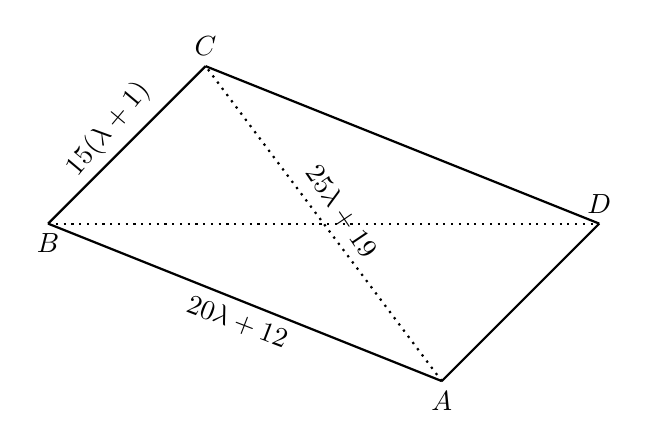
\begin{tikzpicture}[scale=1]
            \coordinate (A) at (5,0);
            \coordinate (B) at (0,2);
            \coordinate (D) at (7,2);
            \coordinate (C) at (2,4);		
            \draw[thick] 	(A) node[below]{$A$} -- node[midway,rotate=-21,below]{$20 \lambda + 12$} 	
            (B) node[below]{$B$};
            \draw[thick] (C) node[above]{$C$} -- 
            (D) node[above]{$D$};
            \draw[thick,dotted] (A) -- node[midway,rotate=-56,above]{$25 \lambda + 19$} (C);
            \draw[thick,dotted] (B) -- (D);
            \draw [thick] (B) -- node[midway,rotate=50,above]{$15(\lambda + 1)$} (C);
            \draw [thick] (A) -- (D);
        \end{tikzpicture}
    \end{center}
    \item 	 \begin{tabbing}
        $ABCD$ est un rectangle	\= $\Leftrightarrow$ $ABC$ est rectangle en $B$\\
        \>	$\Leftrightarrow AC^2=AB^2+BC^2 \quad$ \textit{d'après le théorème de Pythagore et sa réciproque}\\
        \> $\Leftrightarrow (25\lambda+19)^2=(20\lambda+12)^2+\left(15(\lambda+1)\right)^2$\\
        \> $\Leftrightarrow 625\lambda^2+950\lambda+361=400\lambda^2+480\lambda+144+225\lambda^2+450\lambda+225$\\
        \> $\Leftrightarrow 625\lambda^2+950\lambda+361=625\lambda^2+930\lambda+369$\\
        \> $\Leftrightarrow 20\lambda=8$\\
        \> $\Leftrightarrow \lambda=\dfrac{8}{20}$\\[0.5em]
        \> $\Leftrightarrow \lambda =\dfrac{2}{5}$
    \end{tabbing}	
    \item	Les diagonales d'un rectangle sont de même longueur.\\
    Donc pour $\lambda=\dfrac{2}{5}$ : $\quad BD= AC = 25\times \dfrac{2}{5}+19=29$
\end{enumerate}


\end{document}